\documentclass[12pt,letterpaper]{article}
\usepackage[utf8]{inputenc}
\usepackage{amsmath,amssymb,fullpage,graphicx}
\usepackage{subfigure}
\let\hat\widehat
\let\tilde\widetilde


\author{Nan Tang\\1662478}
	%% your name
\title{STAT 403 Spring 2018\\HW06}
	%% title of this document
\begin{document}
\maketitle
	%% make the title and author

\section*{Q1}
\subsection*{Q1-1}
\noindent Since bootstrap samples are taken with replacement from sample $X_1, X_2, ... X_n$, for each value $X_i$ in bootstrap sample,
\begin{align*}
P(X_i = X_1) = P(X_i = X_2) ... = P(X_i = X_n) = \frac{1}{n}
\end{align*}
\noindent The CDF of $X_i$ can be written as 
\begin{align*}
F_{X_i}(x) &= P(X_i \leq x) \\
&= \sum_{k=1}^{n} P(X_i = x_k) \text{, where } x_k \leq x \text{, and } x_k \in {x_1, x_2, ... x_n} \\
&= \frac{1}{n} \sum_{k = 1}^{n} I(x_k \leq x)
\end{align*}

\noindent The CDF of $X_i$ is same as $\hat{F_n}(x)$, the EDF of original data set. Therefore we can conclude that the bootstrap sample is an IID from EDF of original data set. 

\subsection*{Q1-2}
\begin{align*}
Var(\bar{X^\star}) &= Var(\frac{1}{n} \sum_{i=1}^{n} X_i ) \text{, since } \bar{X^\star} = \frac{1}{n} \sum_{i=1}^{n} X_i \\
&= \frac{Var(\sum_{i=1}^{n} X_i)}{n^2} \text{, by property of variance} \\
&= \frac{\sum_{i=1}^{n} Var(X_i)}{n^2} \\
&= \frac{Var(X)}{n} \\
\text{Note that  } Var(X) &= \frac{1}{n} \sum_{i=1}^{n} (X_i - \bar{X})^2 \\
Var(\bar{X^\star}) &= \frac{\sum_{i=1}^{n}(X_i - \bar{X})^2}{n^2}
\end{align*}

\begin{align*}
S_n^2 &= \frac{1}{n-1} \sum_{i=1}^{n} (X_i - \bar{X})^2 \\
(n - 1) S_n^2 &= \sum_{i=1}^{n} (X_i - \bar{X})^2 \\
Var(\bar{X^\star}) &= \frac{(n-1) S_n^2}{n^2}
\end{align*}

\noindent As $n \rightarrow \infty$, $\frac{n - 1}{n^2} \rightarrow n$. Therefore, when bootstrap sample size is large enough, variance of bootstrap sample mean is equal to $\frac{S_n^2}{n}$.

\newpage
\section*{Q2}
\subsection*{Q2-a}
\begin{verbatim}
origin_sd <- sd(faithful$waiting)
bt_size <- 10000
sample_size <- length(faithful$waiting)
bt_result <- rep(NA, bt_size)

for (ii in 1:bt_size) {
  index <- sample(sample_size, sample_size, replace=T)
  bt_dt <- faithful$waiting[index]
  bt_result[ii] <- sd(bt_dt)
}

hist(bt_result, probability=T, col='cornflowerblue', xlab='SD',
     ylab='Density', main='Histogram of Bootstrapped sample SD')
abline(v=origin_sd, lwd=3, lty=1, col='coral1')
\end{verbatim}

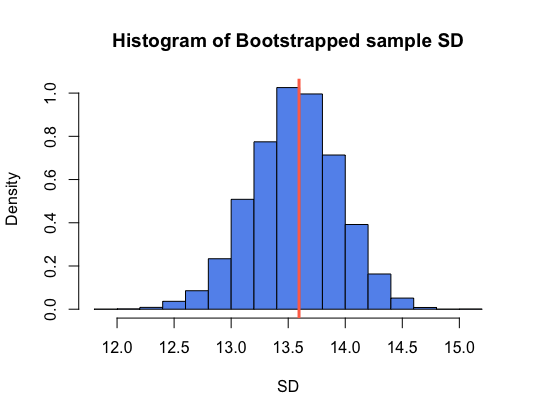
\includegraphics[width=150mm]{hist_bt_sd.png}

\subsection*{Q2-b}
\begin{verbatim}
bt_var <- sd(bt_result)^2
bt_mse <- mean((bt_result - origin_sd)^2)
> bt_var
[1] 0.147665
> bt_mse
[1] 0.1488451
\end{verbatim}

\noindent Variance of sample SD is 0.147665, and MSE is 0.1488451. 

\subsection*{Q2-c}
\begin{verbatim}
bt_sd <- sd(bt_result)
lower_bd <- origin_sd + qnorm(0.975) * bt_sd
upper_bd <- origin_sd - qnorm(0.975) * bt_sd
> lower_bd
[1] 14.34813
> upper_bd
[1] 12.84181

> quantile(bt_result, c(0.025, 0.975))
    2.5%    97.5% 
12.78565 14.30731 
\end{verbatim}

\noindent By theorem, the $95\%$ confidence interval is $[12.84181, 14.34813]$. In bootstrap samples, $95\%$ interquantile is $[12.78565, 14.30731 ]$.

\subsection*{Q2-d}

\begin{align*}
\text{p-value} &= \text{P(getting value more extreme than sample SD} | H_0)
\end{align*}

\noindent Since the bootstrap sample sd follows normal distribution, we may assume the sampling distribution is normal with $\mu_0 = 15$ and $\sigma = $ bootstrap standard deviation. 

\begin{verbatim}
bt_sd <- sd(bt_result)
p_value <- 2 * pnorm(origin_sd, 15, bt_sd)

> p_value
[1] 0.0002558503
\end{verbatim}

\subsection*{Q2-e}
\noindent The variance of bootstrapped samples is $\frac{\sigma^2}{n}$, indicating the value will decrease as sample size increases. Larger sample size
minimizes the margin of error, of which smaller margin of error makes the estimation more accurate. 

\section*{Q3}
\subsection*{Q3-a}
\noindent Regular bootstrap method to get MSE
\begin{verbatim}
admission_dt <- UCBAdmissions[,,1]
origin_or <- (admission_dt[1,1] * admission_dt[2,2]) / 
  (admission_dt[2,1] * admission_dt[1,2])

n_male <- admission_dt[1,1] + admission_dt[2,1]
n_female <- admission_dt[1,2] + admission_dt[2,2]
n <- n_male + n_female

male_dt <- c(rep(1, admission_dt[1,1]), rep(0, admission_dt[2,1]))
female_dt <- c(rep(1, admission_dt[1,2]), rep(0, admission_dt[2,2]))

bt_ep_or <- rep(NA, N)
for (ii in 1:N) {
  male_index <- sample(n_male, n_male, replace=T)
  female_index <- sample(n_female, n_female, replace=T)
  sp_male <- male_dt[male_index]
  sp_female <- female_dt[female_index]
  male_adm <- sum(sp_male)
  male_reject <- n_male - male_adm
  female_adm <- sum(sp_female)
  female_reject <- n_female - female_adm
  sp_or <- (male_adm * female_reject) / (male_reject * female_adm)
  bt_ep_or[ii] <- sp_or
}

> bt_ep_mse
[1] 0.008787036
\end{verbatim}

\noindent The MSE of bootstrap OR is 0.008787036.

\newpage
\subsection*{Q3-b}
\noindent $H_0$: no gender bias exists (OR = 1)\\
\noindent $H_1$: gender bias exists (OR $\neq$ 1)
\begin{align*}
\text{p-value} &= \text{P(getting value more extreme than 0.3492} | H_0)
\end{align*}

\noindent We may use standard deviation of bootstrap sample as an estimator of sampling distribution standard deviation. 

\begin{verbatim}
bt_ep_sd <- sd(bt_ep_or)
p_value <- 2 * pnorm(origin_or, 1, bt_ep_sd)

 p_value
[1] 3.589365e-12
\end{verbatim}

\noindent The p-value of this test is $3.589365 \times 10^{-12}$. \\

\noindent To test this hypothesis, we may also apply permutation test. 
\begin{verbatim}
data_pull <- c(rep(1, admission_dt[1,1] + admission_dt[1,2]), 
               rep(0, admission_dt[2,1] + admission_dt[2,2]))

N <- 10000
bt_per_or <- rep(NA, N)
for (ii in 1:N) {
  sp_index <- sample(n, n, replace=T)
  sp_dt <- data_pull[sp_index]
  sp_male <- sp_dt[1:n_male]
  sp_female <- sp_dt[(n_male+1):n]
  male_admit <- sum(sp_male)
  male_reject <- length(sp_male) - male_admit
  female_admit <- sum(sp_female)
  female_reject <- length(sp_female) - female_admit
  sp_or <- (male_admit * female_reject) / (male_reject * female_admit)
  bt_per_or[ii] <- sp_or
}
\end{verbatim}

\noindent Since the bootstrap OR follows normal distribution, we may assume the sampling distribution is normal. 

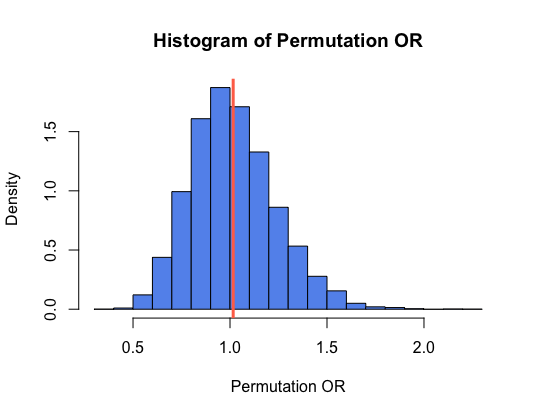
\includegraphics[width=150mm]{hist_per_or.png}

\begin{verbatim}
bt_per_sd <- sd(bt_per_or)
p_value <- 2 * pnorm(origin_or, 1, bt_per_sd)

> p_value
[1] 0.002984116
\end{verbatim}

\noindent The p-value of permutation test is $0.002984116$.

\newpage
\subsection*{Q3-c}
\noindent In this problem, we generated data based on parameters: number of male rejected, admitted, and number of female rejected, admitted. \\
\noindent Let $\theta_1$ denotes male admission rate, and $\theta_2$ denotes female admission rate. 
\begin{align*}
\theta_1 &= \frac{\# \text{male admitted}}{\# \text{total male applicants}} \\
\theta_2 &= \frac{\# \text{female admitted}}{\# \text{total femalte applicants}}
\end{align*}

\noindent For both empirical and parametric bootstrap approaches, each bootstrap sample has probability of $\theta_1$ or $\theta_2$ to be admitted and $(1 - \theta_1)$ or $(1- \theta_2)$ to be rejected, since bootstrap is with replacement. Therefore, both empirical and parametric bootstrap samples should follow same distribution. i.e. empirical and parametric approaches are same procedure in this problem. 




%%% do not touch anything below
\end{document}
